\section{Theoretical Analysis}
\label{sec:analysis}

\paragraph{}
THIS IS NOT ACTUAL
In this section, we can find the results of each topic required in the theoretical analysis. The numeric results or graphics are presented alongside a short explanation of the interpretation of the problem. All of the results were obatined usig GNU octave and the section is dividid in six different subsections - Subsection ~\ref{subsec:first_topic}, Subsection ~\ref{subsec:second_topic}, Subsection ~\ref{subsec:third_topic}, Subsection ~\ref{subsec:fourth_topic}, Subsection ~\ref{subsec:fifth_topic} and Subsection ~\ref{subsec:sixth_topic} -, one for each topic of the theoretical analysis.

\[
\left\{\begin{matrix}
v_t=v_n+v_f\\
f = 1 kHz = 1000 Hz \\
NEED TO BE IMPROVED
A=14;
T=1/50;
t=linspace(0, T/2, 1000);
%linspace(base,limit,n);
w=2*pi*(1/T);
R=1000
C=100e-6
\end{matrix}\right.
\]

%%%%%%%%%%%%%%%%%%%%%%%%%%%%%%%%%%%%%%%%%%%%%%%%%%%%%%%%%%%%%%%%%%%%%%%%%%%%%%%%%
\subsection{Envelope Detector Circuit}
\label{subsec:envelope}

\paragraph{}
The voltage source $v_S$ produces a sinusoidal wave and is defined by the following expression: $v_S=Acos(\omega t)$.

The envelope detector circuit includes a full-wave bridge rectifier, whose voltage output $v0_{rect}$ corresponds to the absolute value of the voltage source $v_S$.

\[
v0_rect =
\left\{\begin{matrix}
v_S, v_S \ge 0\\
-v_S, v_S \le 0\\
\end{matrix}\right.
\]

Finally, the envelope detector circuit voltage $v_0$ is the highest between $v0_rect$, the full-wave bridge rectifier voltage, and the voltage $v0_{exp}$ induced when the capacitor $C$ discharges through the resistor $R$, described by the following equation: $vO_{exp}=Acos(\omega t_{OFF})e^(\frac{-({tON}-{tOFF})}{RC})$.

\begin{figure}[H] \centering
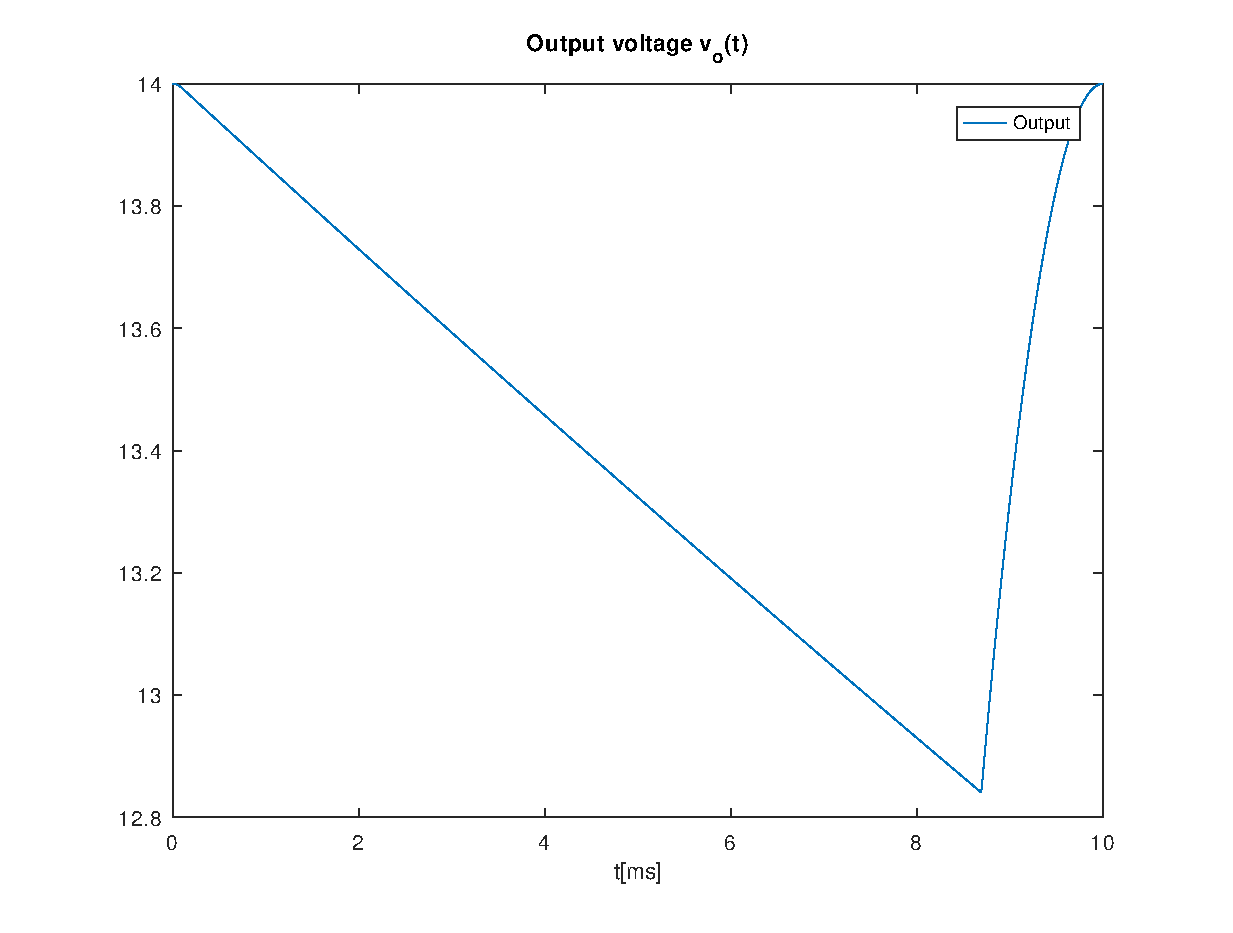
\includegraphics[width=0.6\textwidth]{envelope.eps}
\caption{The final envelope detector circuit voltage $v_0$ during a half-period interval.}
\label{fig:envelope}
\end{figure}

where $t$ is expressed in miliseconds (ms) along the x-axis and 
$v_0)$, the envelope output voltage, is expressed in Volts (V) along the y-axis.
%%%%%%%%%%%%%%%%%%%%%%%%%%%%%%%%%%%%%%%%%%%%%%%%%%%%%%%%%%%%%%%%%%%%%%%%%%%%%%%%%%%%

\subsection{Voltage Regulator Circuit}
\label{subsec:regulator}

The voltage regulator attenuates oscillations in the input signal without frequency dependence and takes advantage of the non-linear characteristic of the $N$ diodes included in the positive voltage limiter. 

The voltage analysis of the regulator applies the incremental analysis method, separating the DC and incremental components.

The diode incremental resistance is calculated using the following expression: $r_d=\frac{\eta v_t}{I_s e^(\frac{v_d}{\eta v_t}}$.

Applying the voltage divider rule, the AC increment $v_{out}$ is defined using the following relation: $vout=\frac{N r_d}{N rd+R2}vO$.

On the other hand, the DC voltage $V_{OUT}$ is obatined multypling the diode voltage $v_d$ by the number of diodes $N$ used in the voltage regulator circuit: $V_{OUT}=N v_d$.

\[
v0_rect =
\left\{\begin{matrix}
NEED TO BE IMPROVED
n=17;
R2=10e3;
eta=1;
vt=25e-3;
vd=0.706;
I_s=1e-14;
\end{matrix}\right.
\]

The final voltage of the regulator circuit $v_{OUT}$ is obtained adding the results of the incremental analysis and the DC analysis: $v_{OUT}=v_{out}+V_{OUT}$.

\begin{figure}[H] \centering
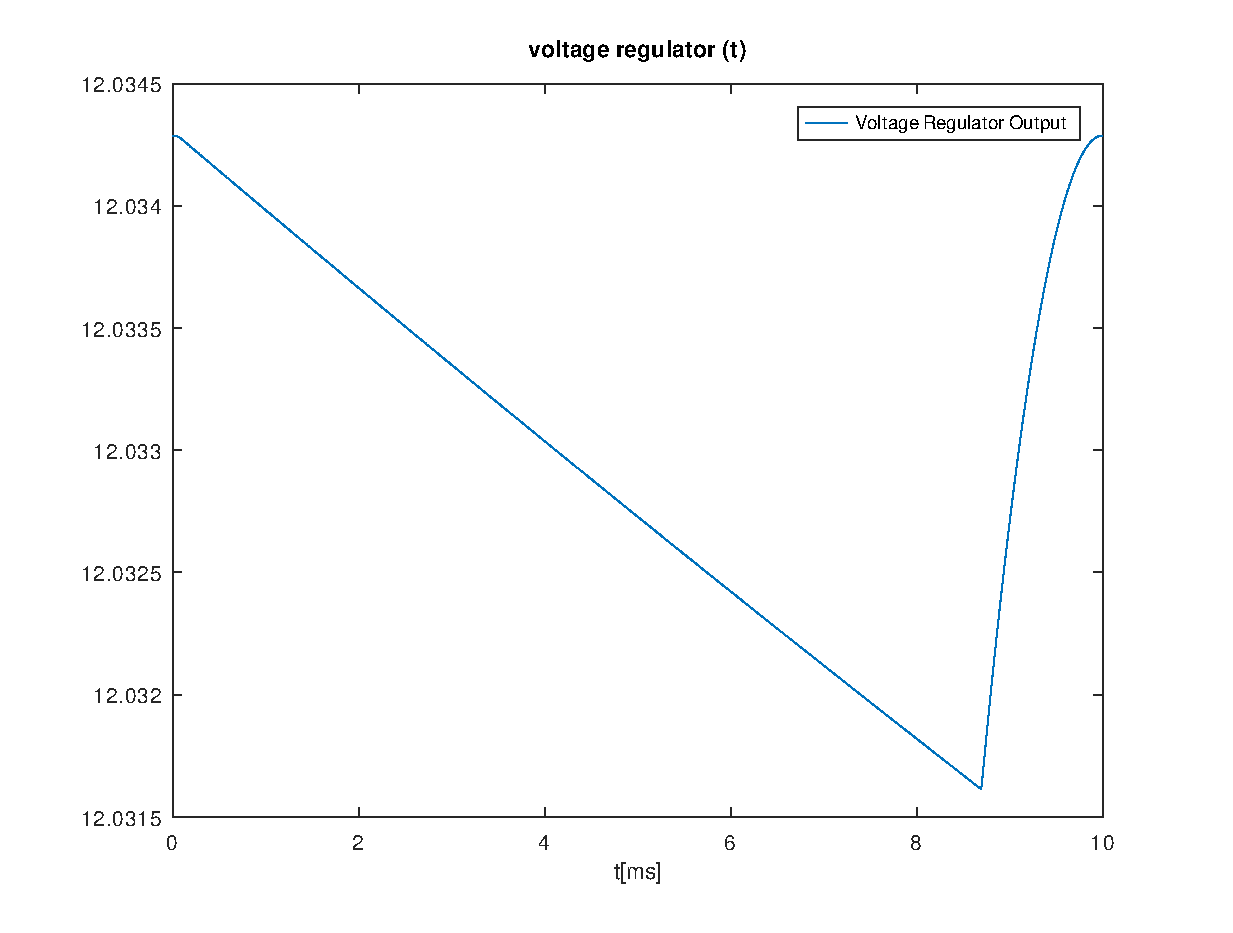
\includegraphics[width=0.6\textwidth]{output.eps}
\caption{The final voltage $v_{OUT}$ of the voltage regulator circuit during a half-period interval.}
\label{fig:output}
\end{figure}

where $t$ is expressed in miliseconds (ms) along the x-axis and 
$v_{OUT}$, the voltage of the regulator, is expressed in Volts (V) along the y-axis.

%%%%%%%%%%%%%%%%%%%%%%%%%%%%%%%%%%%%%%%%%%%%%%%%%%%%%%%%%%%%%%%%%%%%%%%%%%%%%%%%%%%%%
\subsection{Voltage Ripple}
\label{subsec:ripple}

The voltage ripple can be improved using a full-wave rectifier circuit in the envelope detector circuit. 

The value of the voltage ripple $v_{ripple}$ can be calculated relating the maximum and the minimum values of the final voltage of the regulator circuit $v_{OUT}$, using the following expression: $v_{ripple}=max(v_{OUT})-min(v_{OUT})$.

\begin{center}
   \begin{tabular}{|c||c|}
      \hline    
      \multicolumn{2}{|c|} {\bf THIS SHOULD PRINT THE RIPPLE BELOW \\
      \hline
        \input{vripple}
   \end{tabular}
 \end{center}

%%%%%%%%%%%%%%%%%%%%%%%%%%%%%%%%%%%%%%%%%%%%%%%%%%%%%%%%%%%%%%%%%%%%%%%%%%%%%%%%%%%%%
\subsection{The Output DC Level}
\label{subsec:dclevel}

The $t_{ON}$ is calculated using the Newton-Raphson iterative method, starting with a function obtained through the following equation: $Acos(\omega t_{ON})=Acos(\omega t_{OFF})e^(\frac{-(t_{ON}-t_{OFF})}{RC})$.

The DC level output average is obtained integrating the sinusoidal and exponential functions during a half-period interval. The calculations are shown below.

$t\in[0,t_{OFF})\\
\int_{0}^{t_{OFF}}=\frac{N r_d}{N r_d + R_2}\frac{A}{\omega}sin(\omega t_{OFF})+N v_d t_{OFF}\\$

$t\in[t_{OFF},t_{ON})\\
\int_{t_{OFF}}^{t_{ON}}=\frac{N r_d}{N r_d + R_2}(-A R C cos(\omega t_{OFF})(e^{\frac{-({tON}-{tOFF})}{RC}}-1))+N v_d (t_{ON} - t_{OFF})$

$t\in[t_{ON},\frac{T}{2)]\\
\int_{t_{ON}}^{\frac{T}{2}}=\frac{N r_d}{N r_d + R_2}\frac{A}{\omega}(sin(\omega \frac{T}{2})-sin(\omega t_{ON}))+N v_d (\frac{T}{2}-t_{ON})$

$\overline{V}=\frac{\int_{0}^{t_{OFF}}+\int_{t_{OFF}}^{t_{ON}}+\int_{t_{ON}}^{\frac{T}{2}}}{\frac{T}{2}}$

\begin{center}
   \begin{tabular}{|c||c|}
      \hline    
      \multicolumn{2}{|c|} {\bf THIS SHOULD PRINT THE AVERAGE BELOW \\
      \hline
        
 THE OUTPUT VOLTAGE AVERAGE LEVEL IS & 12.0248 V \\ \hline 
   \end{tabular}
 \end{center}

The Output DC Level accuracy can be evaluated through comparing the final voltage of the circuit $v_{OUT}$ and the $12 V$ constant function. 

\begin{figure}[H] \centering
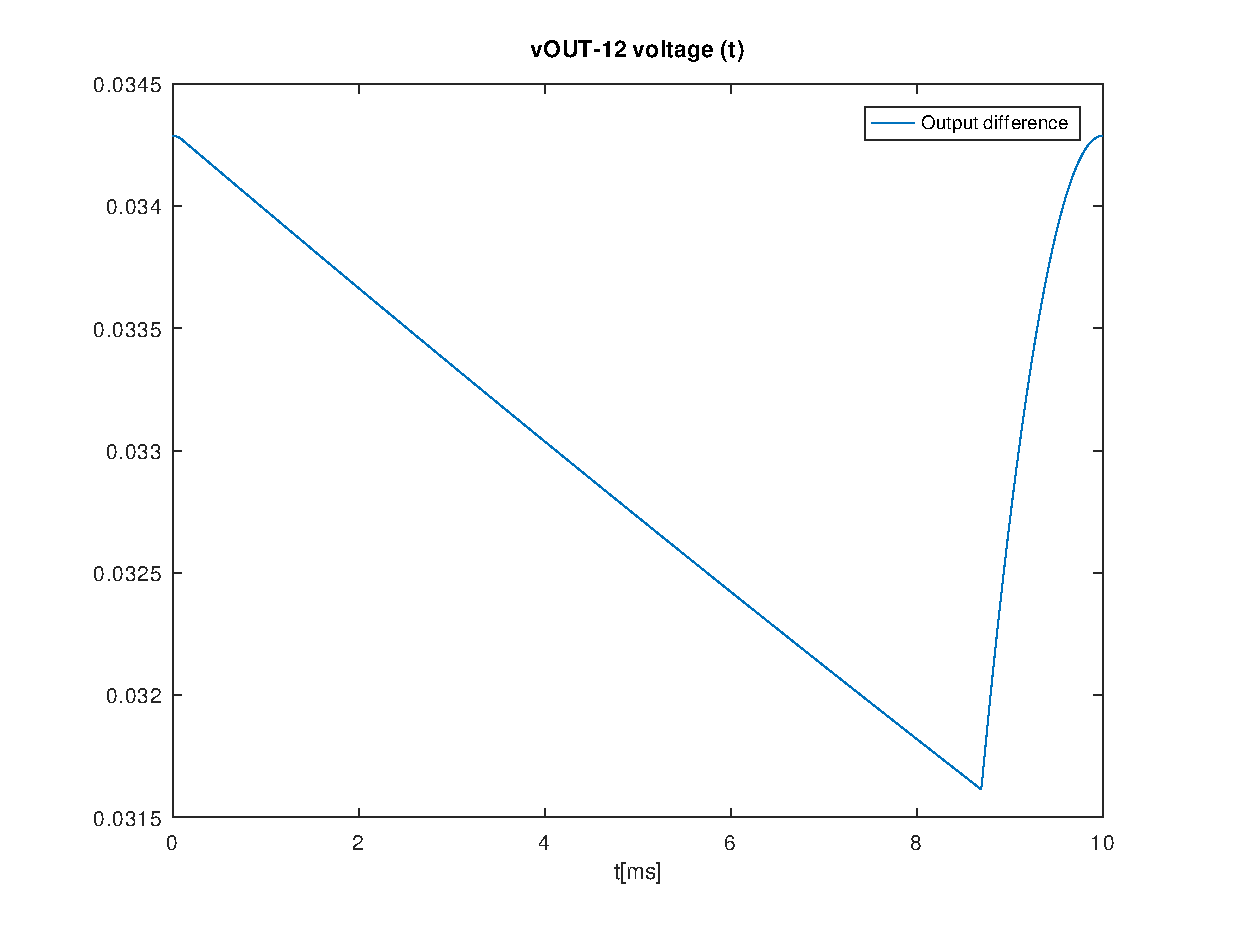
\includegraphics[width=0.6\textwidth]{outputdiff.eps}
\caption{The voltage $v_{OUT}-12$ during a half-period interval.}
\label{fig:outputdiff}
\end{figure}

Where $t$ is expressed in seconds (s) along the x-axis and 
$v_{OUT}-12)$, the output voltage difference, is expressed in Volts (V) along the y-axis.
